\documentclass[12pt, a4paper]{article}
\usepackage[english]{babel}
\usepackage[T1]{fontenc}
\usepackage[utf8]{inputenc}
\usepackage{mathtools}
\usepackage{amsfonts,amsmath,amssymb,amsthm}
\usepackage{enumerate}
\usepackage[margin=.5in]{geometry}
\usepackage{fouriernc}
\usepackage{listings}
\usepackage{multirow}
\usepackage[table]{xcolor}
\usepackage{booktabs}

\title{ACOTSP}
\author{Stanisław Bitner - 438247}
\date{\today}

\begin{document}
\maketitle

\section*{Implementations}

The general idea is as follows:
\begin{itemize}
    \item calculate choice info values described in the paper;
    \item construct $N$ tours ($N$ is the number of cities);
    \item update pheromone as described in the paper;
    \item find the best tour.
\end{itemize}

Last step is not strictly necessary, but it is useful for debugging purposes,
such as tracking changes of the best tour's length.\\
It is also worth mentioning that before starting the algorithm we start by
setting up curand states and calculating $\eta^\beta$ values for all edges.
Also, the initial $\tau$ is set to $1$ as it proved to be the best choice.\\
Note that in order to fully grasp the ideas described below it might be better
to also look at the code.

\subsection*{Floating point precision}

Precision of floating point numbers turned out to be a major problem. To battle
this, I scale all the edges by the maximum distance in the graph (only for
calculating probabilities). What's more, the pheromone traces are exponentially
decaying, so they quickly reach very small values that are rounded to zeros.
Due to this, the ants are unable to find a new path. Therefore, I set a fixed
lower bound. The last difficulty would be that comparison of close floating point
numbers leads to weird results, therefore I allow a small error margin.

\subsection*{Choice info update}

The array \emph{choice\_info} is updated by $N^2$ threads in parallel. Each
thread is responsible for a single edge. To slightly improve performance, I use
\emph{\_\_powf} function instead of \emph{powf}, as suggested in the paper.
Thread/block layout is $N$ blocks of $N$ threads, or rather $1024$ blocks of
$1024$ threads, which is the upper bound of $N$.

\subsection*{Worker ant tour construction}

There is $N$ blocks with a single thread working in parallel. There is no
synchronization between threads, as they are all independent and the global
values they read are unfortunately accessed in a random order. Each thread
constructs a single tour, which is first stored in registers and then written
to global memory. Instead of using a tabu list, I decided to store the cities
in a single array \emph{tour}. First \emph{step} elements are the cities
already visited in order, and the rest are the numbers of cities not yet
visited at random. This allows to reduce the number of cities to look at as the
ones not visited are stored in a contiguous memory segment. When visiting a
city, \emph{choice info} is put into local memory. Then the sum of
probabilities is calculated. Then each ant selects a probability from a uniform
distribution and finds first city such that the cumulative probability is
greater than the selected one. In the event that floats get messed up and no
such city is found, the city is chosen basically at random.\\
Both tour and read values of \emph{choice info} are stored in the shared
memory. It reduces the read/write times. This is also the reason we spawn $N$
blocks with $1$ thread, rather than $1$ block with $N$ threads.

\subsection*{Queen ant tour construction}

$N$ blocks of $N$ threads are used to construct the tours. Each block
represents a queen commanding $N$ ants. Each ant is responsible for its own
city. Tabu list is implemented as a single boolean value for each thread. In
the shared memory, I store \emph{choice info} values, their sum, tour and
random probability.\\
In each step ants read \emph{choice info} values into shared memory. Then a
single thread decides a random probability from a uniform distribution.\\
Afterward an exclusive scan is performed on the \emph{choice info} values.
Each index of the array is shifted by an adequate offset to prevent memory bank
conflicts. The sum is equal to value of last element before plus value of last
element after scan.\\
Then each ant divides its \emph{choice info} value by the sum and checks if the
chosen probability fits in its range (with epsilon margin). If it does, the
city is selected as a candidate for the next city. It is important to note that
I divided the values instead of multiplying the random probability, because
otherwise floats got to zero.\\
Afterward the next city is chosen non-deterministically amongst the candidates
(thus separate runs, might yield different results, even with the same seed).
There might be many such candidates originally because of the epsilon margin
and float precision.\\
Then the ant responsible for the selected candidate sets its \emph{tabu} value
to true and its city as the next one in the tour.\\
At the end tour is written to global memory ($k$-th thread writes the $k$-th
visited city).

\subsection*{Pheromone update}

Same layout as in the choice info update.\\
First one kernel multiplies $\tau$ by $1 - \rho$, but does not go below a fixed
lower bound.\\
Afterward to compute length of each tour, tours are put into shared memory --
1 tour per block. Then a reduction is performed on the weights of the edges
(also in shared memory).\\
As mentioned before I scale the lengths by the maximum distance in the graph
and then increment $\tau$ using atomic adds.\\
One may wonder use atomic operations instead of doing scatter to gather or
something like a parallel histogram. The reason is simple, it's because it's
faster. Standard scatter to gather requires $N^2$ operations per thread, which
is unacceptable.\\
As for the parallel histogram -- it sounds great, but has too big constant
overhead. One possible way of doing it would be as follows:
\begin{itemize}
    \item store edges in order $(i_0,j_0),(i_1,j_1,\ldots$;
    \item reorder them to $(0,j_0),(1,j_1),\ldots$;
    \item transpose matrix obtained matrix:
        \[
            \begin{pmatrix}
                (0,j_{0,0}) & \ldots & (0,j_{0,{n-1}}) \\
                \vdots & \ldots & \vdots \\
                (n-1,j_{n-1,0}) & \ldots & (n-1,j_{n-1,n-1})
            \end{pmatrix}
        \];
    \item sort rows by $j$ values;
    \item perform enum operation to get segments for reduction on each row;
    \item reduce segments and add perform at most one add per edge.
\end{itemize}
This process sounds fine and has just $\mathcal{O}(\log n)$ time complexity,
but unfortunately it has a very big constant factor, which is the reason I
chose to stick with atomic operations. Worst case is much worse, but on average
it is much faster.\\
All in all, tests have proven that the implementation with atomic adds is the
fastest of the 3 mentioned above.

\subsection*{Best tour finding}

There is a single block of $N$ threads. Each thread is responsible for a single
tour length. A reduction is performed on pairs $(C,k)$, where $C$ is the length
of the $k$-th tour, and $k$ is the index of the tour and also the index of the
thread. A standard min reduction is performed and the index of the shortest
tour is stored.

\section*{Performance}

\begin{table}[h]
    \centering
    \caption{Average execution times (ms.) on Titan V for ACOTSP implementations.}
    \scalebox{0.8}{
        \begin{tabular}{|l|c|c|c|c|c|c|}
            \hline
            Code & \multicolumn{6}{c|}{TSPLIB codes (problem size)} \\
            \cline{2-7}
            version & \( d198 \) & \( a280 \) & \( lin318 \) & \( pcb442 \) & \( rat783 \) & \( pr1002 \) \\
            \hline
            1. Worker & $2.36 \pm 0.69$ & $4.74 \pm 0.42$ & $5.47 \pm 0.18$ & $11.59 \pm 0.86$ & $37.73 \pm 0.30$ & $102.62 \pm 1.86$ \\
            \hline
            2. Worker Graph & $2.33 \pm 0.90$ & $4.69 \pm 0.43$ & $5.42 \pm 0.19$ & $11.53 \pm 0.79$ & $37.71 \pm 0.31$ & $101.51 \pm 1.63$ \\
            \hline
            3. Queen & $2.55 \pm 0.82$ & $4.76 \pm 0.14$ & $5.41 \pm 0.93$ & $11.18 \pm 0.90$ & $32.97 \pm 0.97$ & $54.78 \pm 0.27$ \\
            \hline
            4. Queen Graph & $2.51 \pm 0.58$ & $4.71 \pm 0.51$ & $5.37 \pm 0.31$ & $11.08 \pm 0.41$ & $31.94 \pm 0.94$ & $52.73 \pm 0.14$ \\
            \hline
        \end{tabular}
    }
\end{table}

Table 1 shows the average execution times for a single iteration all algorithms
for different problem sizes. The collected results show the averages and
standard deviations of 1000 runs.

Below, I present the benchmarks for all the kernels implemented in the
solution (pheromone update stages are counted as a single kernel).

\begin{table}[h]
    \centering
    \caption{Average execution times (ms.) on Titan V for different kernels.}
    \scalebox{0.8}{
        \begin{tabular}{|l|c|c|c|c|c|c|}
            \hline
            Kernel & \multicolumn{6}{c|}{TSPLIB codes (problem size)} \\
            \cline{2-7}
                   & \( d198 \) & \( a280 \) & \( lin318 \) & \( pcb442 \) & \( rat783 \) & \( pr1002 \) \\
                   \hline
            1. update choice info & $0.13 \pm 0.39$ & $0.18 \pm 0.43$ & $0.17 \pm 0.34$ & $0.27 \pm 0.40$ & $0.62 \pm 0.17$ & $0.97 \pm 0.23$ \\
            \hline
            2. worker tour construction & $2.29 \pm 0.68$ & $4.67 \pm 0.42$ & $5.39 \pm 0.18$ & $11.49 \pm 0.84$ & $37.56 \pm 0.30$ & $102.38 \pm 1.84$ \\
            \hline
            3. queen tour construction & $2.48 \pm 0.28$ & $4.68 \pm 0.37$ & $5.33 \pm 0.25$ & $11.87 \pm 0.27$ & $32.80 \pm 0.47$ & $54.54 \pm 0.27$ \\
            \hline
            4. pheromone update & $0.16 \pm 0.25$ & $0.19 \pm 0.28$ & $0.21 \pm 0.28$ & $0.27 \pm 0.28$ & $0.63 \pm 0.38$ & $0.97 \pm 0.39$ \\
            \hline
            5. find best tour & $0.58 \pm 0.24$ & $0.57 \pm 0.19$ & $0.60 \pm 0.18$ & $0.56 \pm 0.20$ & $0.62 \pm 0.26$ & $0.62 \pm 0.25$\\
            \hline
        \end{tabular}
    }
\end{table}

\newpage

\section*{Results}

\begin{figure}[ht]
    \centering
    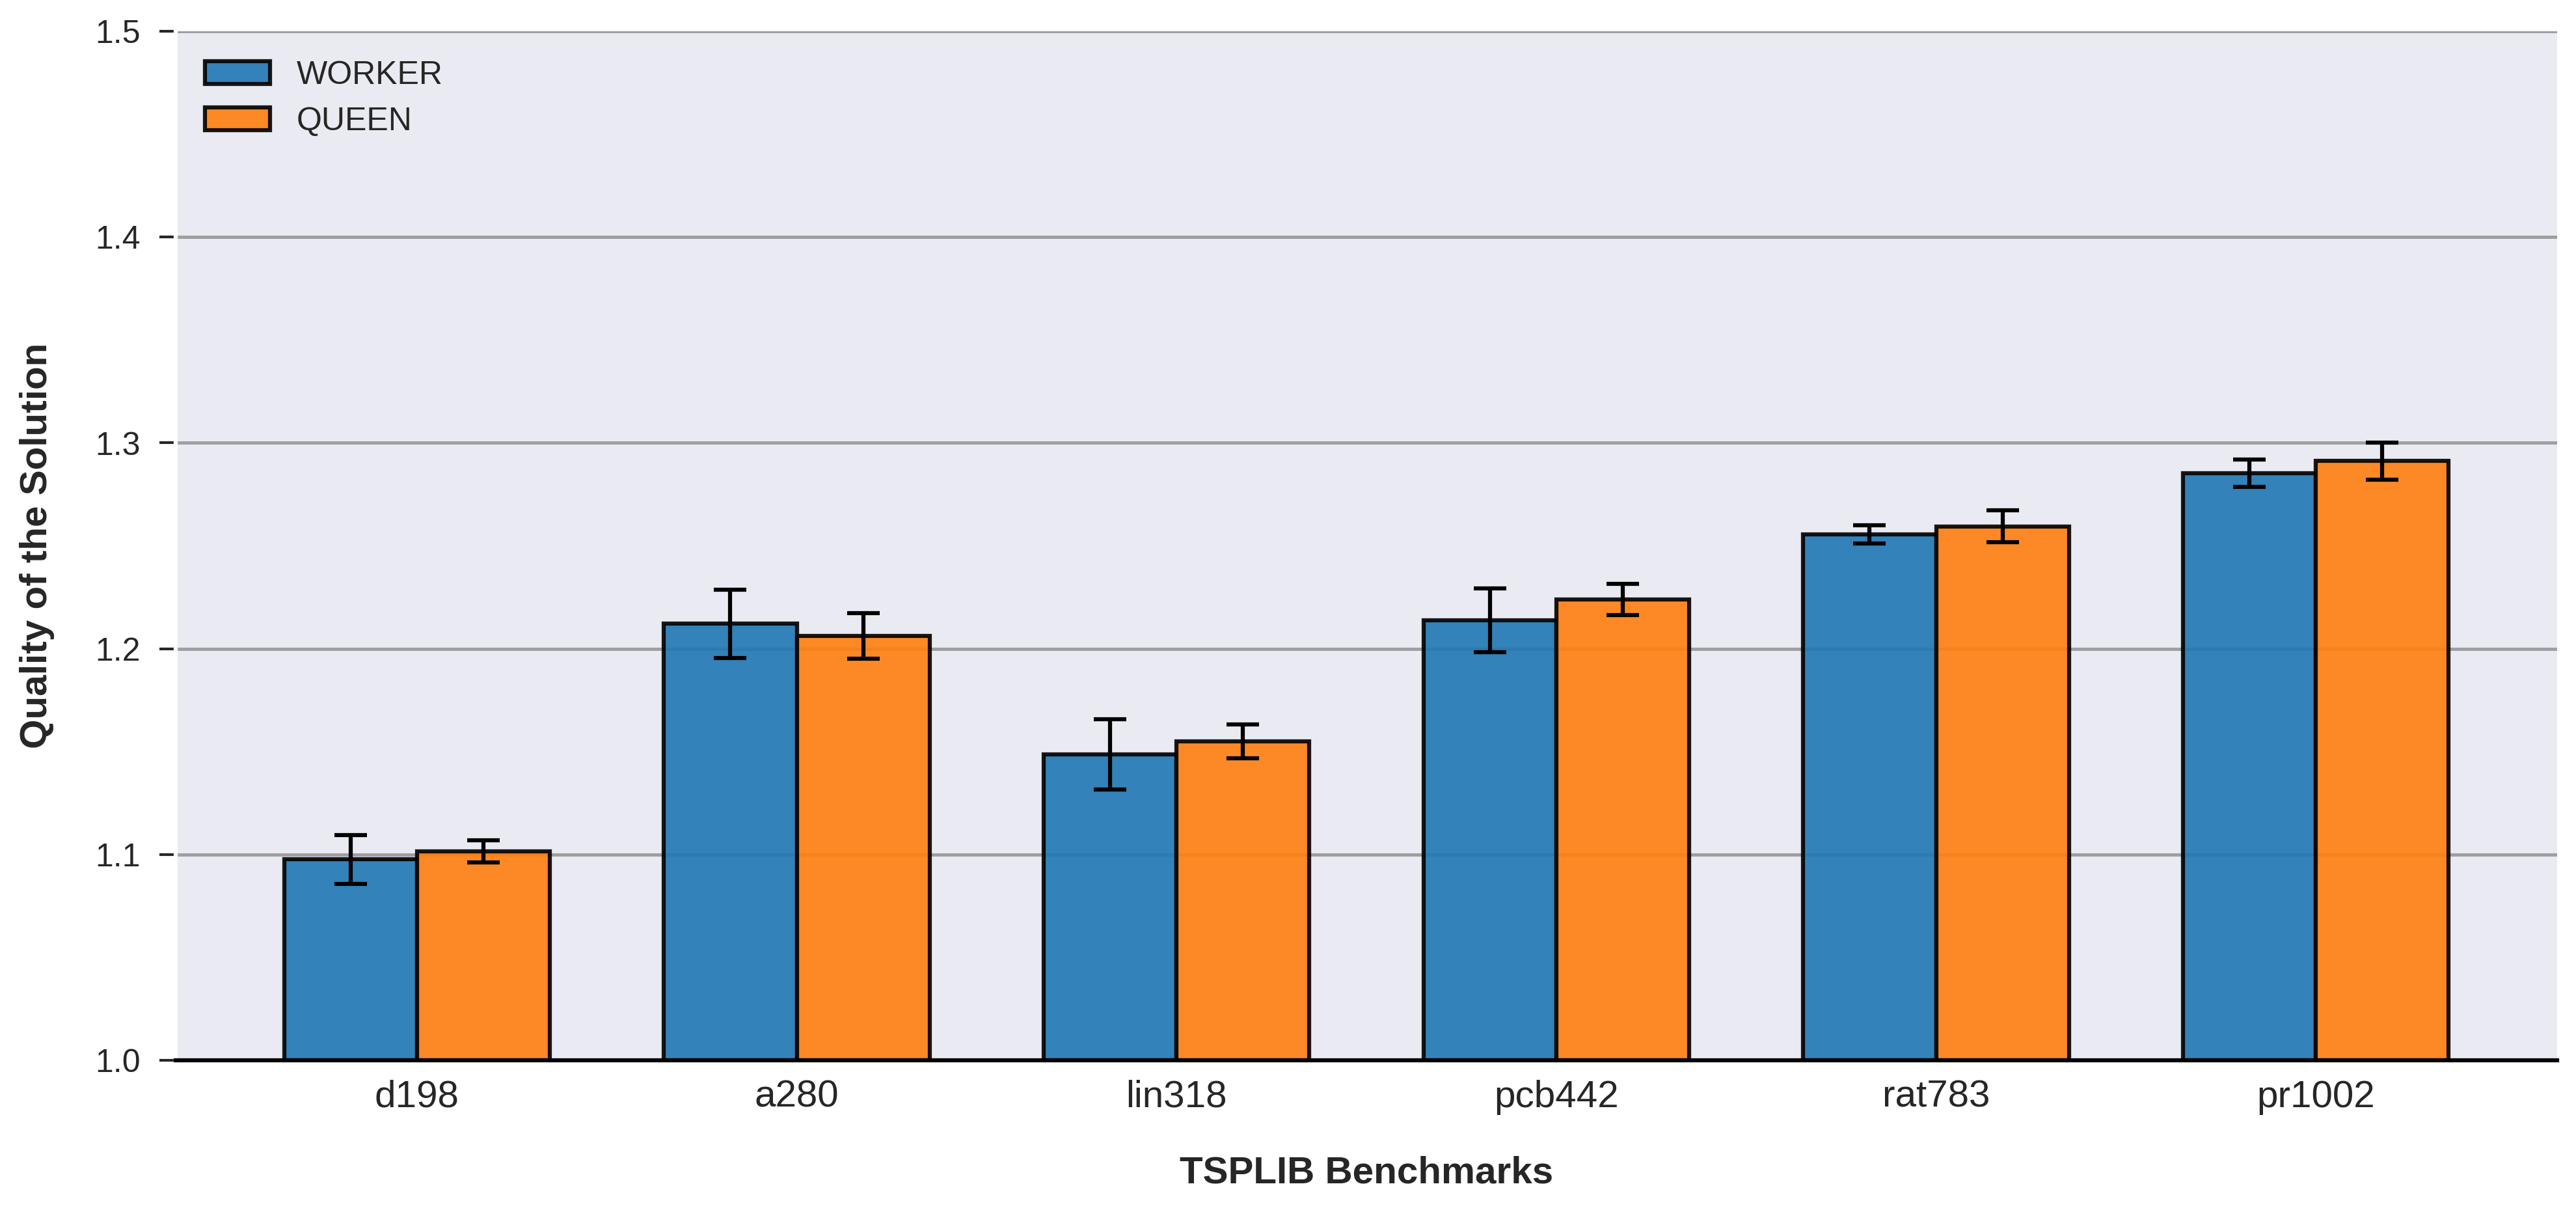
\includegraphics[width=0.8\textwidth]{./performance_comparison.png}
    \caption{Solution quality comparison.}
\end{figure}

Figure 1 depicts a quality comparison for \emph{worker} and \emph{queen} ant
approach. The results have been obtained from running the algorithms a fixed
number of 1000 iterations and averaged over 5 independent runs with different
seeds. Main conclusion would be that both algorithms obtain very similar
results. On average the results fit in the given bounds, however some outliers
occur. Do note that the results are not the tours given in the last iteration,
but the best tours amongst all iterations. They generally get gradually better,
but it is not monotonic descent, thus it is better.

\section*{CUDA features outside the lecture scope}

There are only CUDA Graphs and curand, but I would assume, they are not
necessary to explain…\\
If they are however, here is the explanation:
cuRand -- a CUDA library for generating high-quality pseudo-random and
quasi-random numbers on NVIDIA GPUs. It provides optimized random number
generators for parallel algorithms.\\
CUDA graphs -- a feature in CUDA that captures sequences of kernels and memory
operations into a graph structure. This reduces launch overheads by submitting
the entire graph at once, improving performance for workloads with repetitive
execution patterns, for few kernels it doesn't really matter though.

\end{document}
